\chapter{Introduction}
\section{Background and research purpose}
In the foreseeable future, the electrification of ocean systems, renewable ocean power sources, and ocean energy networks will be necessary, which will help accelerate the growth and deployment of ocean renewable energy and ways to explore and understand the ocean [1]. To achieve electrification in the ocean, it is necessary to deploy corresponding sensor networks underwater and process the data received by underwater sensors in a timely manner. At the same time, underwater sensors are also an essential tool for studying the marine environment. They can easily and flexibly explore underwater terrain and ecological environment, which provides convenience for the deployment of underwater sensor networks. An excellent underwater AUV needs to have good equipment waterproofness, long-distance underwater controllability, and power durability. For the water-resistance of the equipment, we can use high-performance waterproof and pressure-resistant materials. The remote controllability needs to solve the problems of long-distance underwater wireless communication. The durability of electrical equipment requires low energy consumption AUV and high-energy batteries or a continuous power supply. Sufficient power supply can keep underwater sensors and AUVs in an efficient and stable working state for a long time. Indirectly, reducing human interference when electrical equipment is working underwater can also improve work efficiency and reduce deployment costs. Therefore, the energy supply for underwater electrical equipment has become a novel research direction. Such methods can solve the energy supply problem of underwater equipment economically and ensure the system to perform long-term and stable work [3].

In traditional marine engineering, power is supplied to underwater equipment through wet plug-in interfaces [4]. For the traditional wet plug interface technology, its high cost, complex docking method, poor safety performance, and easy to be corroded by seawater, make its disadvantages in marine engineering increasingly obvious. Wireless Power Transfer (WPT) simplifies the connection between underwater equipment and power supply, reduces the continuous operating cost of underwater equipment, saves a lot of resources, and gradually gains the favor of scholars.

The ocean itself and its surroundings contain a lot of energy, such as tidal energy, wave energy, ocean current energy, sea temperature difference energy, and sea salt difference energy. Ocean energy is rich, widely distributed, clean, and pollution-free, but low energy density and strong regionality. These advantages make it attractive as grid-connected energy, and may also make it an isolated and remote ocean energy source, thereby providing a valuable source of ocean space. Continuous development provides power solutions that are attractive. The rapid development of distributed ocean energy applications (such as underwater sensor networks, ocean sensors and monitoring technologies, ocean automatic network buoys, and deep-sea and tsunami buoys) is beneficial. In particular, it can power an autonomous underwater vehicle (AUV) whose service life is limited by its battery power.

\begin{figure}[htbp]
    \centering
    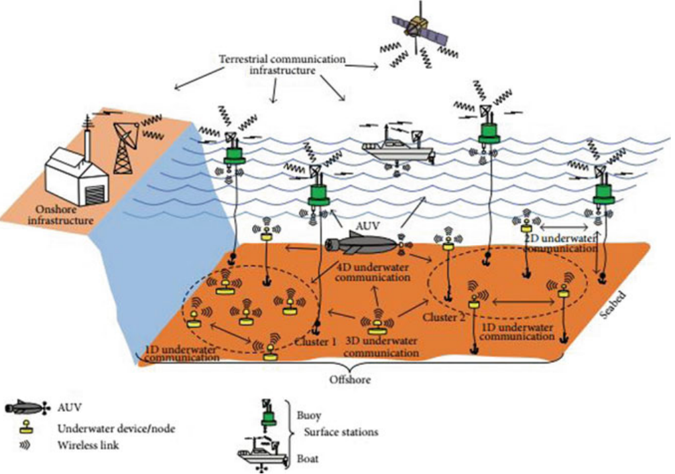
\includegraphics[width=0.7\linewidth]{images/1_underwater_sensor_networks.png}
    \caption{Underwater sensor networks architecture \cite{Nayyar}.}
\end{figure}

% \begin{figure}[htbp]
%     \centering
%     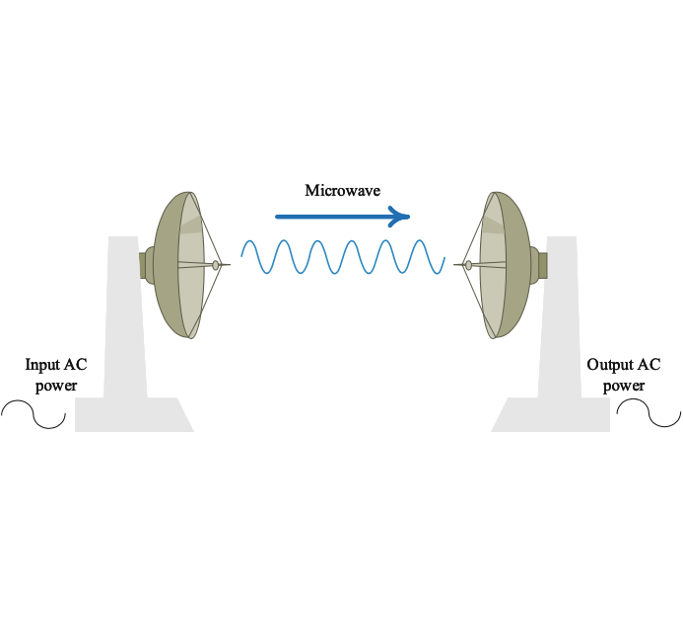
\includegraphics[width=150pt]{images/1_microwave_power_transfer.png}
%     \caption{Microwave power transfer.}
% \end{figure}
% \begin{figure}[htbp]
%     \centering
%     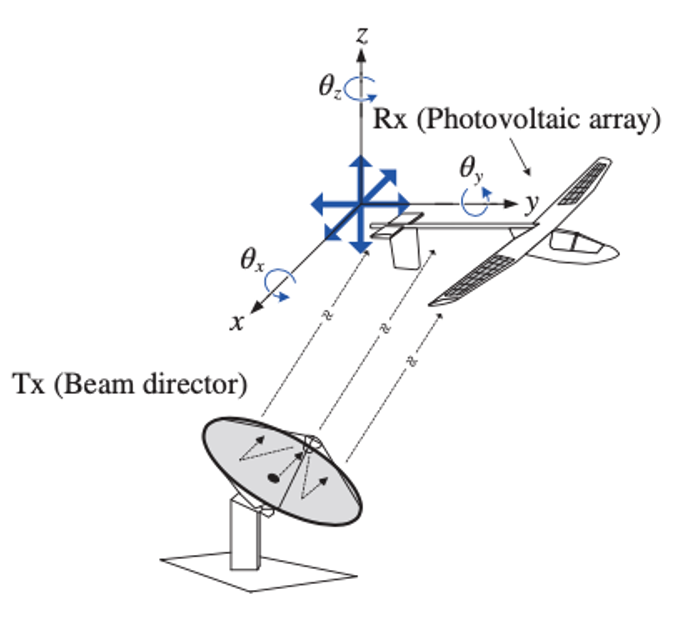
\includegraphics[width=150pt]{images/1_laser_power_transfer.png}
%     \caption{Laser power transfer.}
% \end{figure}


\section{Wireless power transfer technologies}

Broadly speaking, power transfer without direct "electrical contact" between the primary and secondary is wireless power transfer. Wireless energy technology can be divided into two main categories, Near-field (nonradiative region) power transfer and Far-field (radiative region) power transfer. 
Near-field means the area within about 1 wavelength ($\lambda$) of the antenna.  The range of near-field devices is conventionally divided into two categories:
\begin{itemize}
    \item  Short range – up to about one antenna diameter: $D_{range} \leq D_{ant}$. This is the range over which ordinary nonresonant capacitive or inductive coupling can transfer practical amounts of power.
    \item Mid-range – up to 10 times the antenna diameter:  $D_{range} \leq 10 D_{ant}$. This is the range over which resonant capacitive or inductive coupling can transfer practical amounts of power.
\end{itemize} 
Far-field or radiative region – Beyond about 1 wavelength ($\lambda$) of the antenna, the electric and magnetic fields are perpendicular to each other and propagate as an electromagnetic wave; examples are radio waves, microwaves, or light waves.
$D_{ant} << \lambda$.

Therefore, long-distance wireless power transmission includes microwave, light, and sound wireless power transfer. Short-distance wireless power transfer includes short-distance magnetic field transmission using inductive coupling or electric field using capacitive coupling transmission. The respective characteristics are shown in the table ~\ref{table:differentWPT}.

\begin{table}[htbp]
    \centering
    \caption{The different wireless power transmission technologies.}
    \begin{tabular}{ |c|c|c|m{3.5cm}<{\centering}|m{3.5cm}<{\centering}| }
        % \thickhline
        \hline
        \textbf{Technology} & \textbf{Range} & \textbf{Frequency}         & \textbf{Antenna devices}                    & \textbf{Applications}                             \\\hline
        % \thickhline
Microwaves          & hm – km        & GHz                        & Parabolic dishes, phased arrays, rectennas  & Satellite, drone aircraft                         \\ \hline
Optical             & dam – km
                    & $\geq$THz      & Lasers, photocells, lenses & Drone aircraft, space elevator                                                                  \\ \hline
Capacitive          & cm – m         & kHz – MHz                  & Metal plate electrodes                      & Smartcards, biomedical implant
\\ \hline
Inductive           & mm – m         & Hz – GHz                   & Tuned wire coils, lumped element resonators & Electric toothbrush, smartphone, electric vehicle
\\ \hline
    \end{tabular}
    \label{table:differentWPT}
\end{table}



\begin{figure}[htbp]
    \begin{subfigure}{0.5\textwidth}
        \centering
        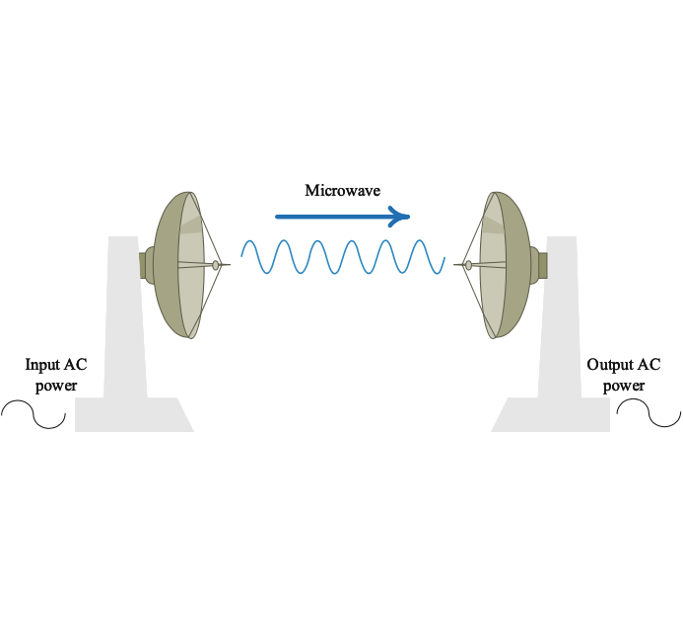
\includegraphics[width=0.9\linewidth]{images/1_microwave_power_transfer.png}
        \caption{Microwave power transfer \cite{Orekan}.}
        \label{fig:subim1}
    \end{subfigure}
    \begin{subfigure}{0.5\textwidth}
        \centering
        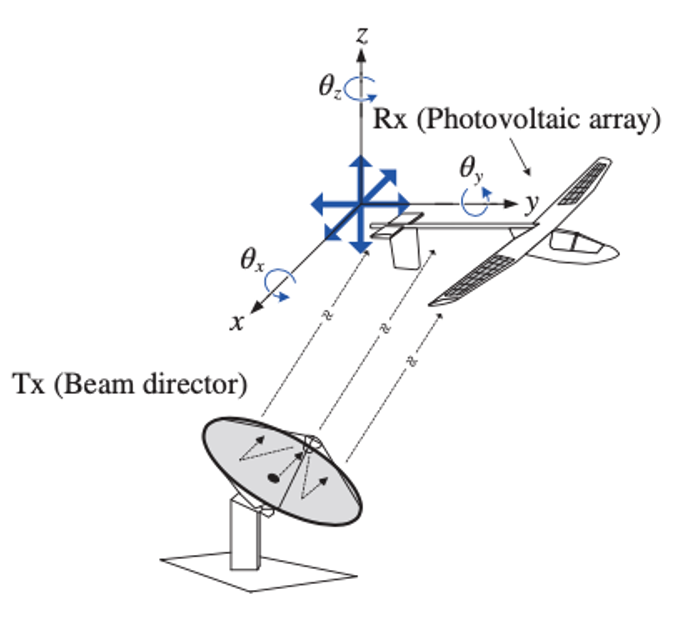
\includegraphics[width=0.9\linewidth]{images/1_laser_power_transfer.png}
        \caption{Laser power transfer \cite{Chun}.}
        \label{fig:subim2}
    \end{subfigure}

    \caption{Far-field wireless power transfer.}
    \label{fig:far-fieldwpt}
\end{figure}

\begin{figure}[htbp]
    \begin{subfigure}{0.5\textwidth}
        \centering
        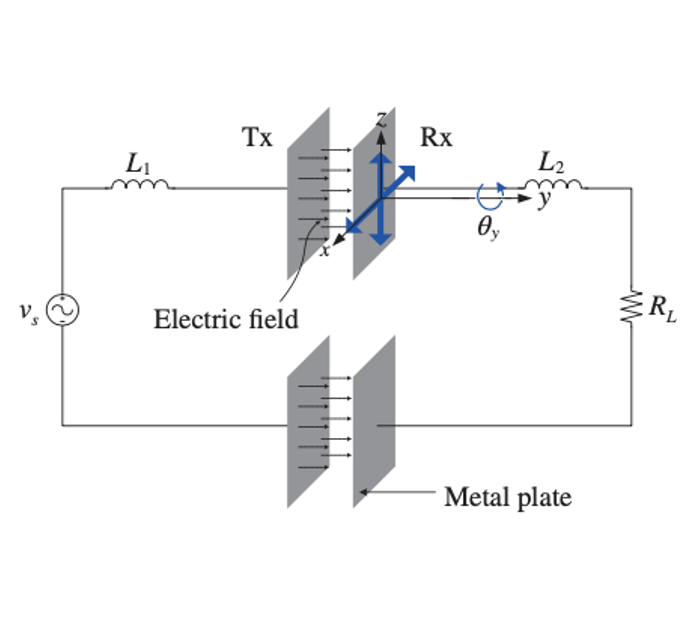
\includegraphics[width=0.9\linewidth]{images/1_capacitive_power_transfer.png}
        \caption{Capacitive power transfer \cite{Chun}.}
        \label{fig:subim1}
    \end{subfigure}
    \begin{subfigure}{0.5\textwidth}
        \centering
        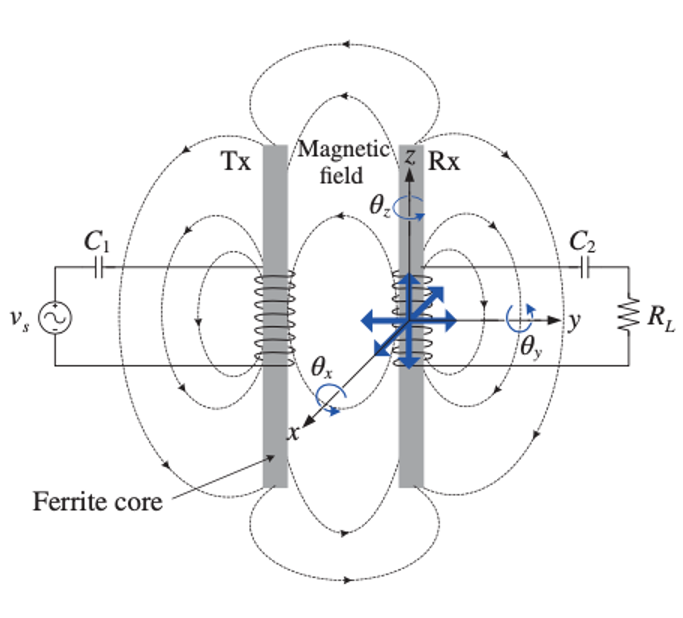
\includegraphics[width=0.9\linewidth]{images/1_inductive_power_transfer.png}
        \caption{Inductive power transfer \cite{Chun}.}
        \label{fig:subim2}
    \end{subfigure}

    \caption{Near-field wireless power transfer.}
    \label{fig:near-fieldwpt}
\end{figure}

\section{Underwater wireless power transfer}
WPT technology has unique advantages in special environments, and along with the continuous development of landing application research and the emergence of a large number of results, it has attracted the attention of underwater technology researchers. As early as 2000, he et al. developed a sub-level rail-type charging device. As shown in the figure, the transmission efficiency is about about. At the same time, the study launched a preliminary discussion on the loss in seawater.
The difference between water and air

Underwater
Seawater has a blocking effect on high-frequency electromagnetic waves. The distance of electromagnetic waves propagating underwater is inversely proportional to the frequency, making it difficult to achieve long-distance power transmission.

Conductivity
Due to the electrical conductivity of seawater, traditional wireless power transmission analysis methods are no longer applicable. At present, the system modeling and related theoretical analysis of underwater wireless power transfer technology need to be improved.

Undercurrent
The submarine landform is complex and there is undercurrent. The coupler core is liable to drift under water, and there are problems such as difficulty in docking, which results in low transmission efficiency.

Other Impact:
Microbial enrichment, temperature, salinity


\section{The main research content of this thesis}
Research on the characteristics of underwater wireless energy transmission.
The design of the underwater wireless energy transmission coil, this research obtained by changing the size, spacing and distribution of the coil
It provides reference materials for the subsequent research on the wpt system of multiple coil groups.

\section{Roadmap}
The first chapter analyzes the background of this research and its research purpose and significance, analyzes the characteristics and advantages and disadvantages of mainstream WPT technology, and provides a basis for using IPT technology as an underwater wireless energy transmission system in the following text. A detailed summary and analysis of the current research status of related technologies at home and abroad, including underwater wired energy transmission technology, WPT technology in underwater and air media, and an explanation of the research focus of this article.

The second chapter focuses on the analysis of the basic theory of wireless energy transmission. The equivalent circuit model and network port model are used to derive the main transmission performance indicators of the system, and the influence of design parameters on the system performance is analyzed to provide theoretical support for subsequent design. Take sea water as an example to simulate the working environment of the system under water. And through simulation software to simulate and analyze related models.

Chapter 3 first analyzes the basic principle of the parallel MRC-WPT circuit, and then based on the WPT model of the ordinary air-core coil, respectively, to address the horizontal offset and angular offset of the transmitter coil and the receiver coil, a new type of battery that can meet the charging requirements is proposed. The wireless energy transmission method of two-dimensional air-core coil and three-dimensional air-core coil enables the transmission efficiency of the underwater MRC-WPT system to be steadily improved. According to the structural characteristics of each method, the corresponding underwater wireless robot model is designed to meet the application conditions.

The fourth chapter first studies the magnetic field characteristics of the air gap coil, focusing on the analysis of the magnetic core's restraining effect on the coil magnetic field, and simulates the magnetic field distribution of the coil containing the air gap core, and proposes a new type of four-phase core coil. The method of wireless energy transmission. By studying the transmitting phase of the four transmitting coils, the induced magnetic fields in the four receiving coils will not cancel each other, and stable energy transmission can be carried out. Then the four-phase magnetic core coil transmission scheme is simulated. Aiming at the characteristics of its magnetic field distribution, the AUV model proposed in the previous article is taken as an example, and a universal application model of the structure is designed under water.